A consequence of separating physics and dynamics grids is that the atmospheric state must be mapped to the physics grid and the physics tendencies must be mapped back to the dynamics grid. Note that tendencies and not an updated state is mapped back to the dynamics grid. If one were to map an updated state the errors in the mapping process may adversely affect the simulation, e.g., in the case of no physics forcing there will be a non-zero `physics forcing' entirely due to the errors in the mapping algorithm.

In a climate model setting it is important that this process does not violate important conservation properties such as:
\begin{itemize}
\item mass-conservation,
\item shape-preserving (monotone), i.e. the mapping method does not introduce new extrema in the interpolated field, in particular, negatives,
\item consistency, i.e. the mapping preserves a constant.
\end{itemize}
Other properties that may be important, but not pursued here, is energy conservation and axial angular momentum conservation. It may be desirable to preserve the high-order of the basis functions during the mapping process so that the mapping is high-order accurate for smooth fields and less information is lost during the mapping process. 


%\begin{equation}
%\psi=\phi_k\, \Delta p_k,
%\end{equation}
%where sub-script $k$ refers to the level index. [conversion back]
\subsection{Remapping state: GLL grid $\rightarrow$ physics grid}
The variables in CAM that are mapped from dynamics to physics grid are: surface pressure $p_s^{(GLL)}$ or pressure-level thickness $\Delta p^{(GLL)}$, zonal velocity component $u^{(GLL)}$, meridional velocity component $v^{(GLL)}$, vertical pressure velocity $\omega^{(GLL)}$, surface geopotential height $\Phi_s^{(GLL)}$, temperature $T^{(GLL)}$, water vapor $Q^{(GLL)}$ and mixing ratios for other scalars $q^{(GLL)}$. In order to achieve conservation of scalar mass and internal energy the remapped variables for scalar mass and temperature is mass-weighted: $\Delta p^{(GLL)}\, q^{(GLL)}$ and $\Delta p^{(GLL)} T^{(GLL)}$, respectively. For more accurate mapping near the poles the velocity vector $(u^{(GLL)},v^{(GLL)})$ in spherical coordinates is transformed into its Cartesian components $(u_x,u_y,u_z)^{(GLL)}$ and mass-weighted. The mass-weighting of the Cartesian velocity vector is to achieve better conservation of axial angular momentum.

\subsubsection{Mapping algorithm}  The mapping procedure follows as a special case of \citet{UT2015MWR}.  Simplified ``first guess'' linear maps associated with each dynamics mesh element are constructed; one first-order monotone and one high-order. For example, the first guess for the high-order map is constructed by integrating the basis functions over the physics grid control volumes using high-order triangular quadrature [{\color{red}{paul: what are we using here?}}]. Each ``first guess'' map is then projected onto the space of conservative and consistent maps using a least squares projection method operating on the coefficients of the linear map. The maps are matrices that can be pre-computed for each element so that the mapping of a field is a matrix operation:
\begin{equation}
\bm{\mathsf{A}}^{(i)}\, \bm{\mathsf{\phi}}=\bm{\mathsf{\psi}}^{(i)},\text{ where }i=`un',`sp', 
\end{equation}
where $\bm{\mathsf{A}}$ is the pre-computed map (matrix) with $np\times np$ columns and $nc\times nc$ rows, superscript `un` and `sp' refers to the unlimited (high-order) map and low-order shape-preserving map, respectively, and $\bm{\mathsf{\phi}}$ is a vector with $np\times np$ rows containing the GLL point values of the field being mapped. The remapped field is in vector $\bm{\mathsf{\psi}}$ that contains $nc\times nc$ rows with physics grid cell average values.

\begin{figure}[t]
\noindent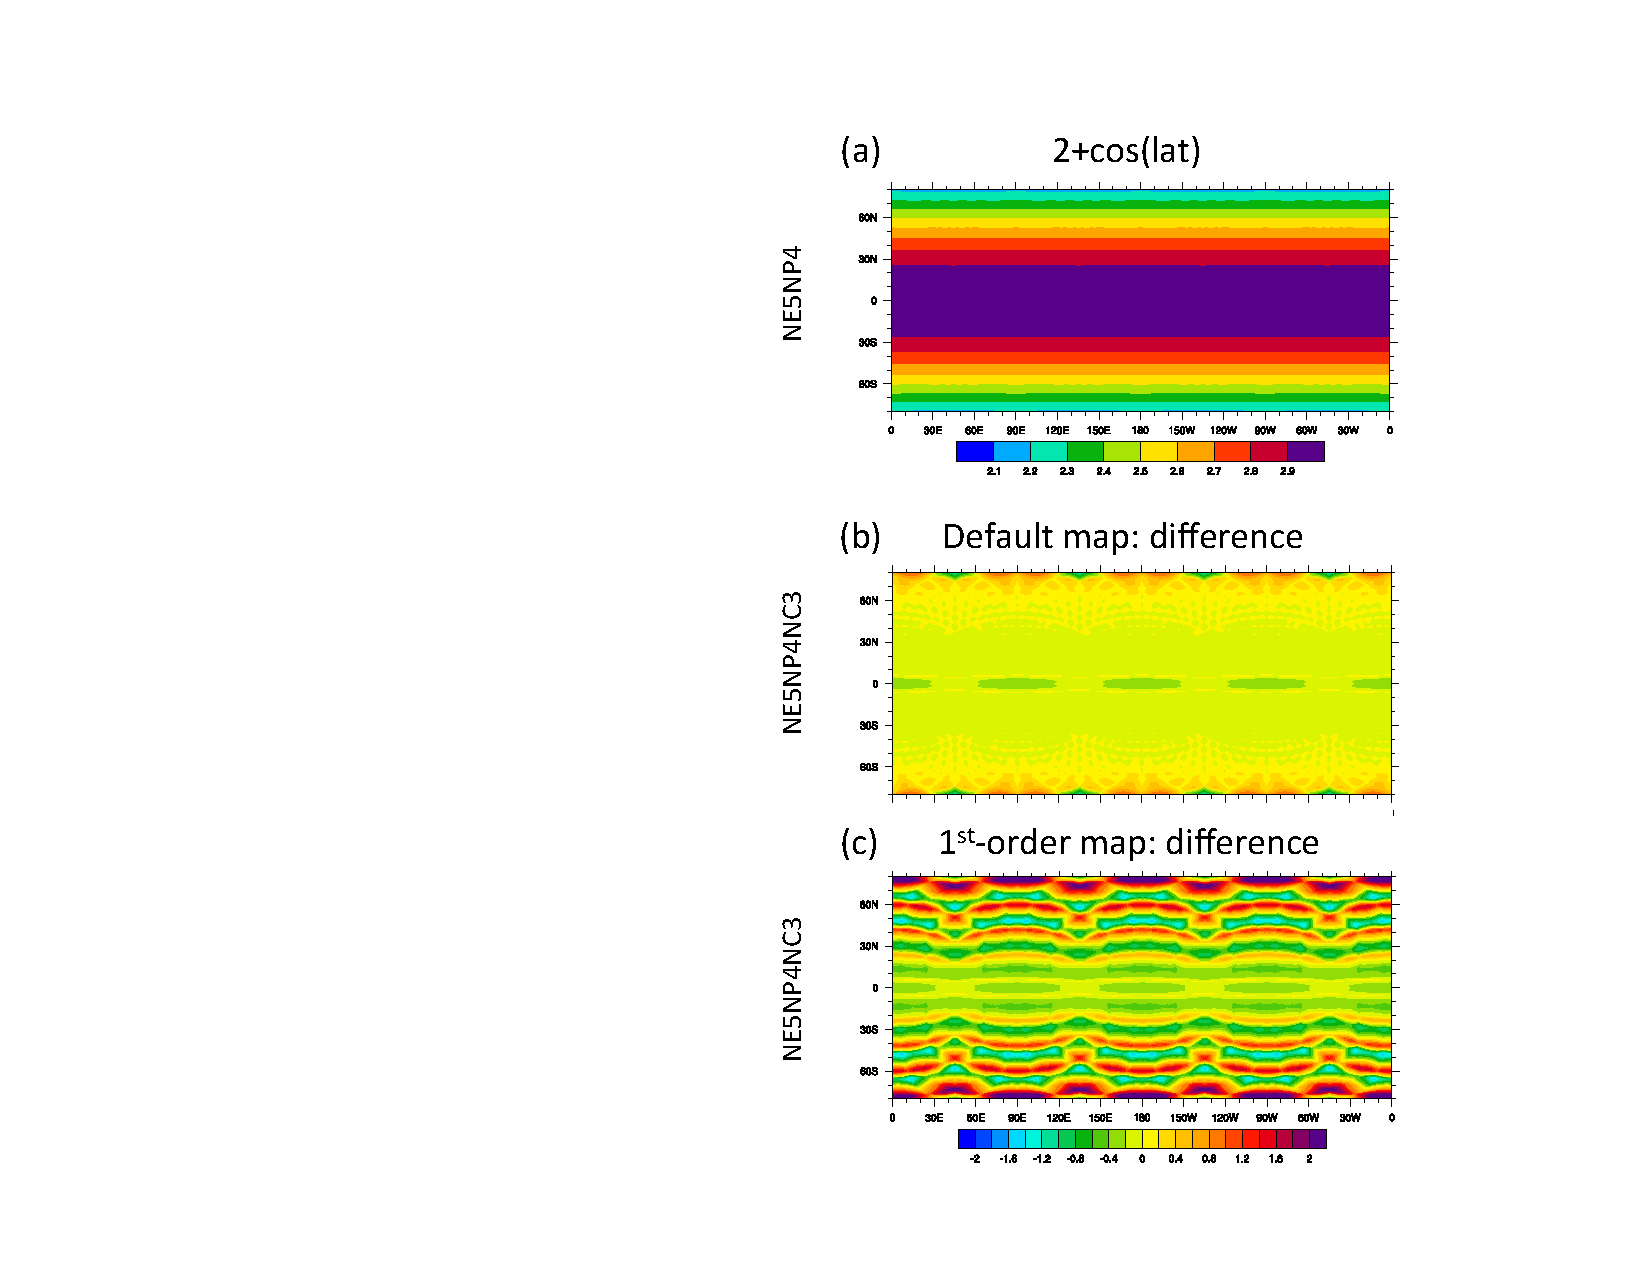
\includegraphics[width=19pc,angle=0]{figs/idealized-mapping-tests-smooth-field.pdf}\\
\caption{(a) Smooth function ($2+\cos(\theta)$) initialized on the $NE5NP4$ GLL grid. (b) and (c) show the difference between the interpolated field and the analytical value at the physics grid cell center. The interpolation is from the $NE5NP4$ GLL grid to the NE5NP4NC3 physics grid (both have an approximate grid spacing of $6^\circ$). In (b) the interpolation algorithm is the default algorithm that is higher-order for smooth fields, shape-preserving, consistent, and mass-conservative. (c) is the same as (b) but using the first-order mapping method. All data has been bilinearly interpolated to a $1^\circ$ regular latitude-longitude grid for plotting.}\label{fig:remap-smooth-field}
\end{figure}
\begin{figure}[t]
\noindent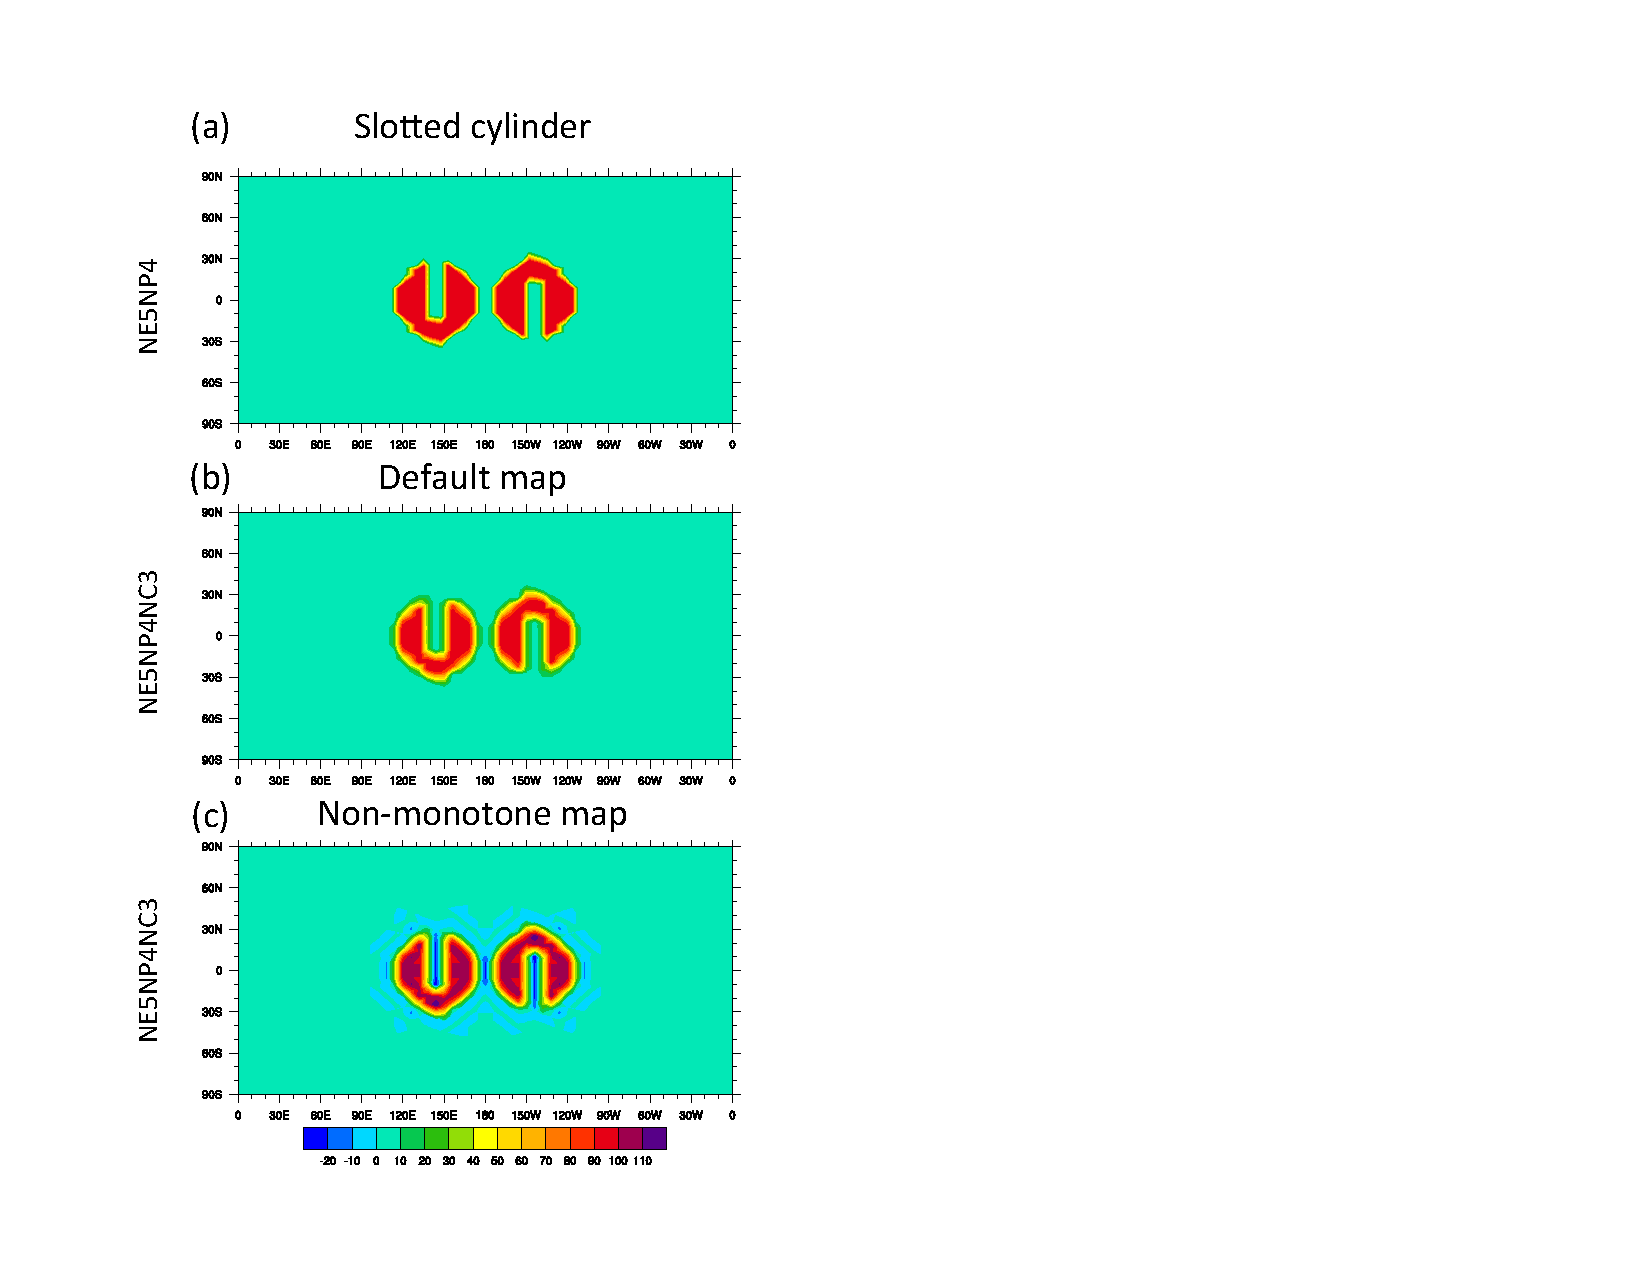
\includegraphics[width=19pc,angle=0]{figs/idealized-mapping-tests-slotted-cylinder.pdf}\\
  \caption{(a) Slotted-cylinder distribution initialized on on the $NE5NP4$ GLL grid (approximately $6^\circ$ resolution). (b) Default mapping of the $NE5NP4$ GLL grid data to the physics grid $NE5NP4NC3$. (c) Same as (b) but using the non-monotone map. All data has been bilinearly interpolated to a $1^\circ\
$ regular latitude-longitude grid for plotting.}\label{fig:remap-slotted-cylinder}
\end{figure}
The low-order map is inaccurate for smooth fields (see Figure \ref{fig:remap-smooth-field}c) and the high-order map is not shape-preserving for, e.g., discontinuous fields (see Figure \ref{fig:remap-slotted-cylinder}c). To avoid using the low-order map in areas where the field is smooth and violation of shape-preservation in areas where the field is not smooth, we linearly combine the two maps in each element:
\begin{equation}
\bm{\mathsf{A}}^{(opt)}=\left[ \alpha^{(opt)} \bm{\mathsf{A}}^{(sp)}+(1-\alpha^{(opt)})\, \bm{\mathsf{A}}^{(un)}\right],\label{eq:opt}
\end{equation}
%so that shape-preservation is not violated and the map retains high-order accuracy where possible.
where $\alpha^{(opt)}$ is the smallest value of $\alpha^{(opt)}$ (so that the high-order map is given as much weight as possible) that guarantees no overshoots or undershoots:
\begin{eqnarray}
\psi_k&\le &\max(\phi_1,...,\phi_{np\times np}), \quad k=1,...,nc\times nc,\label{eq:overshoot}\\
\psi_k&\ge &\min(\phi_1,...,\phi_{np\times np}), \quad k=1,...,nc\times nc.\label{eq:undershoot}
\end{eqnarray}
The value of $\alpha^{(opt)}$ is computed as follows. Assume that there is an overshoot for physics grid cell $k$. We wish to find the value of $\alpha_k$ so that
\begin{equation}
\alpha_k \psi_k^{(sp)}+(1-\alpha_k) \psi_k^{(un)}=\max(\phi_1,...,\phi_{np\times np}),
\end{equation}
which yields
\begin{equation}
\alpha_k = \frac{\max(\phi_1,...,\phi_{np\times np})-\psi_k^{(un)}}{\psi_k^{(un)}-\psi_k^{(sp)}}.
\label{eq:alpha}
\end{equation}
If the absolute value of the denominator in \eqref{eq:alpha} is less than $1.0^{-12}$ then $\alpha_k$ is set to 1. Similarly we compute $\alpha_k$ for undershoots and if there is no under- or over-shoot we set $\alpha_k=0$. The optimal value of $\alpha_k$ that satisfies \eqref{eq:overshoot} and \eqref{eq:undershoot} for all $k$ is
\begin{equation}
\alpha^{(opt)}=\max(\alpha_1, ...,\alpha_{nc\times nc}).
\end{equation}
By optimal we mean the value of $\alpha$ that gives most weight to the unlimited (high-order) map within an element without violating shape-preservation \eqref{eq:overshoot} and \eqref{eq:undershoot}. Note that the linear combination of linear maps is conservative and consistent hence the optimal map \eqref{eq:opt} is conservative, consistent and, by using $\alpha^{(opt)}$, shape-preserving. The limiting process is somewhat similar to \citet{BJ1989} and the flux-corrected transport algorithm \citep{Z1979JCP}.

The mapping of the state variables $\phi$ on the GLL grid to the physics grid is given by
\begin{multline}
\bm{\mathsf{\psi}}=\left[ \alpha^{(opt)} \bm{\mathsf{A}}^{(sp)}+(1-\alpha^{(opt)})\, \bm{\mathsf{A}}^{(un)}\right] \bm{\mathsf{\phi}},
\end{multline}
where $\phi=$ $\Delta p^{(GLL)}$, $\Delta p^{(GLL)}T^{(GLL)}$, $\Delta p^{(GLL)}u_x^{(GLL)}$,$\Delta p^{(GLL)}u_y^{(GLL)}$,$\Delta p^{(GLL)}u_z^{(GLL)}$, $\Delta p^{(GLL)}Q^{(GLL)}$, $\Delta p^{(GLL)}q^{(GLL)}$. The mapped field for, e.g., $\Delta p^{(GLL)}$ is denoted $\psi=\Delta p^{(phys)}$ and similarly for the other variables. The state of the atmosphere is recovered by dividing the mapped fields $\psi$ with pressure-level thickness on the physics grid $\Delta p^{(phys)}$. Since the atmospheric state is mapped from dynamics to physics grid by basically integrating the high-order basis functions, the loss of accuracy is minimized.
%
%
\subsection{Remapping: physics grid $\rightarrow$ GLL grid}
The CAM physics package returns tendencies for temperature $f_T^{(phys)}$, velocity components $(f_u,f_v)^{(phys)}$, water vapor $f_Q^{(phys)}$, other tracers $f_q^{(phys)}$, and surface pressure $f_{PS}^{(phys)}$. The latter forcing is due to the vertical coordinate in CAM-SE being based on `wet' pressure (dry air mass plus the weight of water vapor) so if there is a change in moisture in the column then the `wet' surface pressure  $PS$ changes whereas the dry air mass (surface pressure) remains constant \citep[see section 3.1.8 `Adjustment of pressure to include change in mass of water vapor' in ][]{CAM5}. 

As for the dynamics to physics grid mapping, conservation is important and we therefore mass-weight the variables being mapped. For that $\Delta p$ on the physics and dynamics grid is needed. Mapping the updated surface pressure on the physics grid to the dynamics grid is not desirable: first of all, if there is no tendency on surface pressure then the mapped surface pressure on the GLL grid will be different from the surface pressure on the GLL grid before calling physics. As mentioned before, this is equivalent to having a spurious forcing on $PS$ entirely due to errors in the mapping algorithm. Secondly, conservation properties will result unless the GLL grid surface pressure is overwritten by the mapped $PS$ from the physics grid to the dynamics grid. To ensure conservation and spurious forcing due to mapping errors the following algorithm is adopted for the mass-weighting.

Let $\Delta p_{phys}$ be the updated pressure level thickness returned by physics. Map water-vapor mass $\Delta p_{phys}\, f_Q^{(phys)}$ from the physics to the dynamics grid using a conservative, consistent, and shape-preserving method (see below) resulting in $\Delta p_{phys}\, f_Q^{(phys)}$. This variable is the surface pressure tendency on the GLL grid, $f_{PS}^{(GLL)}$. Now take the surface pressure on the GLL grid before calling physics $p_s^{(GLL)}$ and add the surface pressure tendency $\Delta t PS^{(GLL)}$. This updated surface pressure $p_s^{(GLL)}$ defines the updated pressure-level thicknesses $\Delta p^{(GLL)}$. We use the physics updated pressure level thickness on the physics grid $\Delta p^{(phys)}$ for the mass-weighting of the physics tendencies $f^{(phys)}_i$, where $i=T$, $Q$, $q$, $u_x$. $u_y$, $u_z$, and $\Delta p^{(GLL)}$ for recovering the tendencies after mapping. The velocity forcing is transformed into a Cartesian coordinate system vector as for the dynamics to physics grid mapping.

\subsubsection{Mapping algorithm} [Paul: we are just using low-order map? would it be easy to switch to higher-order?] To build the non-monotone ``first guess'' map from the finite volume physics grid to the finite element dynamics grid, a continuous polynomial reconstruction of degree $n_c-1$ (and order $n_c$) is built that exactly interpolates the volume averaged values in each physics grid element.  For the monotone ``first guess'' map, a second-order bilinear reconstruction is instead employed that interpolates the density field at the center of each finite volume.  In each case the reconstruction is then sampled at each of the Gauss-Lobotto-Legendre nodes of the dynamics grid.

\section{Results}
\begin{figure}[t]
\noindent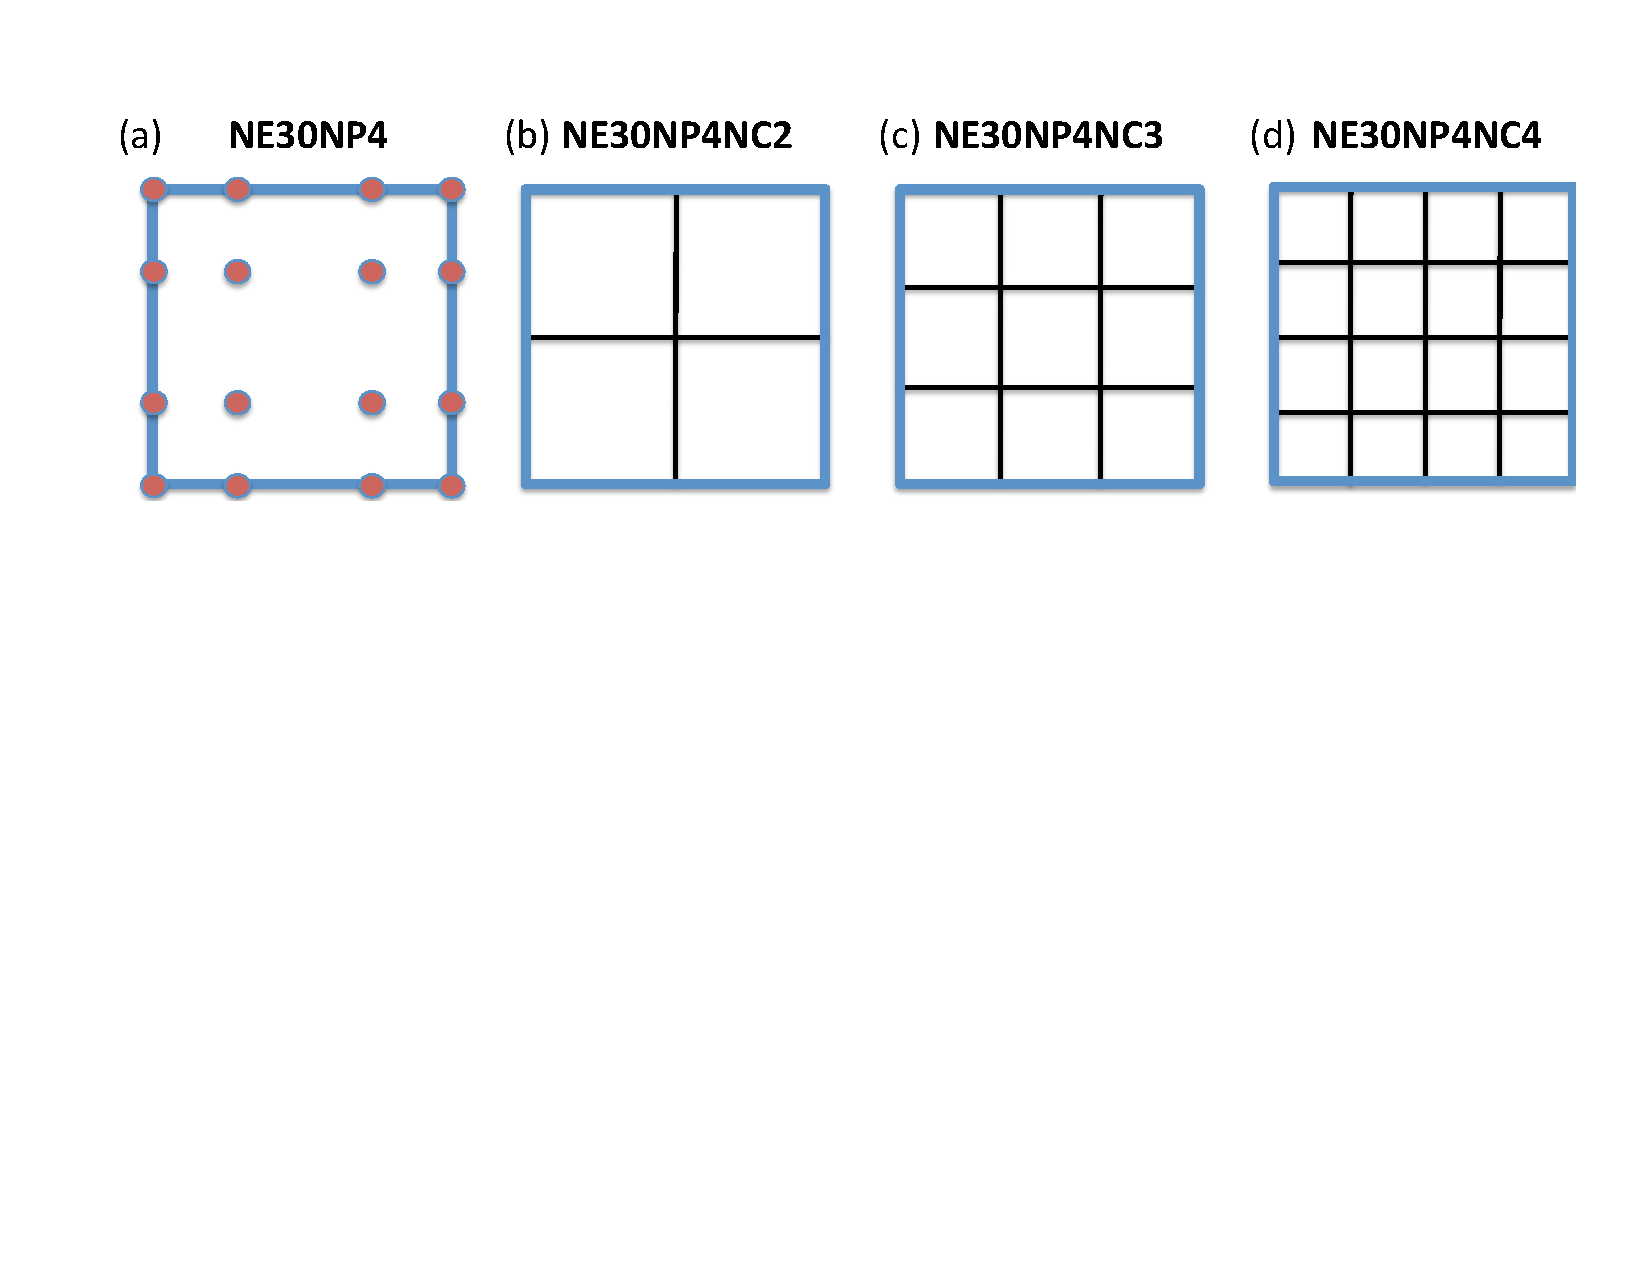
\includegraphics[width=19pc,angle=0]{figs/grids.pdf}\\
  \caption{A graphical illustration of the different physics column configurations: (a) Gauss-Lobatto-Legendre quadrature grid for $np=4$ (filled circles) and (b-d) `equal-area' finite-volume grids of different resolutions ($nc=2,3,4$).}\label{fig:grids}
\end{figure}
%vs
